\chapter{Performance}\label{chapter:Performance}
In the context of high-performance computing, where computational performance and efficiency are crucial, it is paramount to analyze every small piece of software used in the cluster.
This is especially important for this thesis, as the \emph{sys-sage} library is designed to be used in complex, heterogeneous high-performance compute clusters with complicated hierarchical hardware topologies.

As such, analyzing the shared memory implementation of this thesis on metrics such as execution time and scalability is unavoidable.

Since the memory footprint of a topology in shared memory is mostly dependent on the size of the topology itself, with little overhead created by the export process,
the memory impact of sharing topologies using this implementation will not be evaluated as part of this thesis.

\section{Execution}
To perform the performance analysis of the \emph{sys-sage} shared memory implementation, a series of sample topologies will be created, each with different compositions of components, DataPaths and attributes.

The different topologies will then be exported into shared memory regions and subsequently imported into the local memory of another process,
measuring import and export times separately.

To investigate the scalability of the implementation, each topology will be evaluated in multiple sizes, adding more components, DataPaths or attribs as needed.

All performance tests will be executed on an Apple M1 processor with 16GB of RAM.
To create a more reliable performance analysis, all topologies will be evaluated multiple times and the average execution times will be calculated.

\autoref{lst:performance_code} shows how the execution time of exporting a topology is measured. In line 1 and 3, the current time is taken before and after the execution of the measured code section.
This is done using \lstinline|std::chrono::steady_clock|, an implementation of a \emph{monotonic} clock, best suited for measuring time intervals \cite{monotonic_clock}.
In lines 5-6, a \lstinline|std::chrono::duration| is created, representing the time elapsed between \emph{time\_start} and \emph{time\_end}, which is the execution time of the measured code region.

%TODO QUOTE
\begin{lstlisting}[language=c++, numbers=left, caption= Measuring the Execution Time, captionpos=b, label={lst:performance_code}]
    auto time_start = std::chrono::steady_clock::now();
    SharedMemory* shmem = export_component(path, topo, pack);
    auto time_end = std::chrono::steady_clock::now();

    std::chrono::duration<double, std::milli> duration =
        time_end - time_start;
\end{lstlisting}

\section{Basic Component Tree}
For the first performance test, a simple component tree without any DataPaths or attribs is created. The component tree consists of an increasing number of components in a straight line of children, similar to a linked list.

\begin{figure}[ht]
    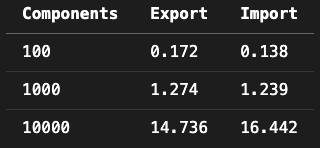
\includegraphics[scale=0.75]{images/component_numbers.png} %TODO Improve graphic, Input real numbers
    \centering
    \caption{Performance Component Tree}
    \label{figure:component_numbers}
\end{figure}

\autoref{figure:component_numbers} shows the execution time in milliseconds of exporting or importing this topology. As expected, the execution time grows linearly with the number of components in the topology.

\section{Attribs}
As complex sys-sage topologies can potentially have a lot of attribs that will often make up a major part of the total data amounts, evaluating the performance of exporting and importing
attribs is paramount to analyzing the performance of the entire system.

\begin{figure}[ht]
    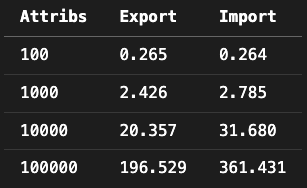
\includegraphics[scale=0.75]{images/attrib_numbers.png} %TODO Improve graphic
    \centering
    \caption{Performance Attrib Topology}
    \label{figure:attrib_numbers}
\end{figure}

\autoref{figure:attrib_numbers} shows the execution time of exporting or importing a topology consisting of a single component, with increasing amounts of attribs.

It is important to note that the performance of sharing complex data attached to an attrib will largely depend on the performance of the \emph{pack} and \emph{unpack} functions provided by the user.
As this factor is impossible to quantify in a meaningful way, the attribs used for the purposes of this performance evaluation are simple integers that don't need to be packed or unpacked.

\autoref{figure:attrib_numbers} shows a linear increase of the execution time with growing number of attribs shared. The performance of export and import are roughly equal, with the import slowing down faster with larger amounts of attribs.

\section{DataPaths}
To test the performance of exporting and importing DataPaths, a small topology consisting of only two nodes is created.
These components are then connected by a large number of DataPaths without attribs or any additional data, so as not to skew the results.

\begin{figure}[ht]
    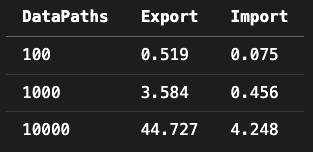
\includegraphics[scale=0.75]{images/dp_numbers.png} %TODO Improve graphic
    \centering
    \caption{Performance DataPath Topology}
    \label{figure:dp_numbers}
\end{figure}

\autoref{figure:dp_numbers} shows the execution time of exporting or importing the topology described above with different amounts of DataPaths.
Apart from some minor fluctuations, the execution time increases roughly linear with the amount of DataPaths in the topology.
The results are as expected, as the DataPaths are simply one after the other, with very little overhead or other performance limiting factors.

It is also notable that importing is consistently almost ten times faster than exporting.
This is likely due to the exporting process needing to evaluate which DataPaths need to be exported, whereas the importing process can directly start importing.